\documentclass[11pt, a4paper, oneside, article]{memoir}
% Setting for memoir
% Set the margins of the document
\setlrmarginsandblock{2cm}{2cm}{*}
\setulmarginsandblock{2cm}{*}{1}
\checkandfixthelayout
\OnehalfSpacing
\captionnamefont{\bfseries\small}
\captiontitlefont{\small}
%\DisemulatePackage{setspace}            % Make sure package is not ignored
%\usepackage[onehalfspacing]{setspace}   % Set the line spacing of the document
%
\usepackage[german, english]{babel}     % Langauge setting
\usepackage[utf8]{inputenc}
\usepackage{graphicx}
\usepackage{wrapfig}                    % Wrapping text arround figures
\usepackage{amsmath}                    % Advanced mathsymbols
\usepackage{chemformula}                % Chemical formulas
\usepackage{pgfgantt}                   % GANTT charts
\usepackage{xcolor}
% Abbreviation glossary
\usepackage[acronym,nogroupskip,nonumberlist,toc]{glossaries}
\setglossarystyle{index}
\makeglossaries                         % Generate the glossary

% Bibliography with biblatex
\usepackage[citestyle=alphabetic,bibstyle=authoryear,citestyle=authoryear,maxbibnames=100,maxcitenames=1,sorting=ynt,backend=biber]{biblatex}
\addbibresource[location=local, datatype=bibtex]{atmo.bib}

\usepackage{csquotes, xpatch}
\usepackage{etex, etoolbox, keyval, ifthen, url} % Needed for chicago-style citations

\chapterstyle{bringhurst}               % Set style for memoir
\graphicspath{{pictures/}}              % Set graphics path

\begin{document}
%Term definitions
% Standard command
%\gls{⟨label⟩}
% Capitalize first letter
%\Gls{⟨label⟩}
% Pluralize term
%\glspl{⟨label⟩}
%Capitalize and pluralize term
%\Glspl{⟨label⟩}

%\newacronym{}{}{}

% Acronyms
\newacronym{voc}{VOC}{Volatile Organic Compound}
\newacronym{bvoc}{BVOC}{Biogenic Volatile Organic Compound}
\newacronym{et}{ET}{evapotranspiration}
\newacronym{npp}{NPP}{Net Primary Production}
\newacronym{odina}{ODINA}{Ozone Damage Interference on Nutrient Allocation}
\newacronym{cuo}{CUO}{Cumulative Uptake of Ozone}
\newacronym{cesm}{CESM}{Community Earth System Model}
\newacronym{clm}{CLM}{Community Land Model}
\newacronym{cam}{CAM}{Community Atmosphere Model}
\newacronym{fun}{FUN}{Fixation and Update of Nitrogen}


\chapter{Research context}
\section{Review of state of the field}
\label{sec:review}

\begin{wrapfigure}[14]{R}[0pt]{0.6\textwidth}
  % R - floating; r - h! [narrow lines] <- reduce whitespace below [17]
  \centering
  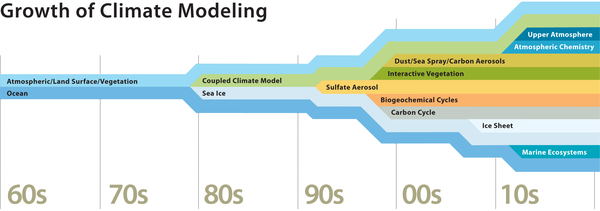
\includegraphics[width=0.58\textwidth]{evolution_of_climate_models}
  \caption{A growth and evolution timeline of climate models. The complexity of global climate models has increased enormously over the last four decades. The most powerful models, such as the \gls{cesm}, now have the capability of simulating a broad range of atmospheric processes, such as the impact of marine ecosystems on the atmosphere. \copyright \gls{ncar}.}
  \label{fig:growth_esm}
\end{wrapfigure}

\textbf{\glspl{esm}} have been rapidly evolving over the past decades (Fig.~\ref{fig:growth_esm}) due to growing computational resources. Over time the scope of the models has substantially broadened and the physical realism of the models has steadily increased, among others due improvements in resolution, grid types, parameterizations and couplers \parencite{AMS:Randall2018}. But this development comes at the cost of a complexity rivaling the real world and immense resources for computing. To predict the response of the Earth’s ecosystem in a changing climate and its feedback on the very same climate, it is important to update model parameterizations to reflect the  state-of-the-art scientific understanding of the underlying processes. From solving the Navier-Stokes equations of wind and waves several decades ago, \glspl{esm} came to represent even biotical process of soil microbial and fungi. But the more we learn the more do we know what is left unknown. At present missing links and knowledge gaps exist especially when it comes to the details of the complex interaction between terrestrial ecosystems and the atmosphere \textbf{\color{red}TODO: Add reference}. First analyses of \gls{cmip}~6 indicate a growing divergence between models \textbf{\color{blue}Added: \parencite{ESD:Tebaldi2021}}, in particular in the land and atmospheric components. Although this will not revoke our fundamental understanding of climate change, it still affects the reliability of model projections.\\

\textbf{The chemical composition of the atmosphere is complex} and the concentration of many important trace gases is highly variable in time and space and substantially influenced by natural and anthropogenic emissions. While increases in the concentrations of well-mixed greenhouse gases such as \ch{CO_2} and \ch{CH_4} are understood as the prime cause of anthropogenic climate warming, anthropogenic activity has also substantially affected the atmospheric concentration of many other chemical species, many of which have important radiative properties.

One of these chemical species is \textbf{ozone, an important trace gas in the lower and middle atmosphere}, and central to this proposal. In accordance with its effects and realm of occurence, we can distinguish the good (stratosphere), \emph{the bad} (troposphere), and \emph{the ugly} (ambient air) ozone throughout the atmosphere. Here we focus on the connection and feedback between the bad and ugly sides of ozone. After \ch{CO_2} and \ch{CH_4}, ozone is ranked third amongst the most potent climate forcers \parencite[Chapter 8]{IPCC2013}. It contributes to warming in the troposphere where it is produced as a secondary air pollutant in chemical cycles involving precursors such as \ch{CO} and \ch{NO_x} as well as hydrocarbons (\gls{voc}, \gls{bvoc}). Ozone is highly toxic and harmful to human health and many ecosystems. Model projections show diverse futures for surface ozone burdens under the \gls{rcp} scenarios, in sign and magnitude strongly dependent on changes in precursor emissions and climate \textbf{\color{red}TODO: Add references: general Reference} \parencites{JGR:Rieder2015}{AE:Rieder2018}{Nat:Skeie2020}. Projections of effects of future ozone air quality on human health and crop damage dependent on the level of ambition in both climate protection and precursor reduction \parencite{PTRS:Schneidemesser2020}.

Despite a successful reduction of precursors in recent years leading to a stagnation of the upward trend in tropospheric ozone concentrations, there are indications that \textbf{climate feedback on the ozone uptake by the land biosphere} can hamper reaching  air quality goals \parencite{NCC:Lin2020}. Under drought conditions, plants will limit their transpiration by closing their stomata, which regulate all of its gas exchange. At the same time, such stressed vegetation is emitting \glspl{bvoc}, an important precursor, and thus increasing ozone concentrations \ch{[O_3]} in ground-level air. As ozone uptake through plants’ stomata is considered one of the most effective removal pathways, stomatal closure under thermal stress will lead to a twofold penalty of climate change on vegetation and air quality. At present however, large uncertainties in non-stomatal removal remain \parencite{RG:Clifton2020}.

\begin{wrapfigure}[26]{R}[0pt]{0.5\textwidth}
  % R - floating; r - h! [narrow lines] <- reduce whitespace below [17]
  \centering
  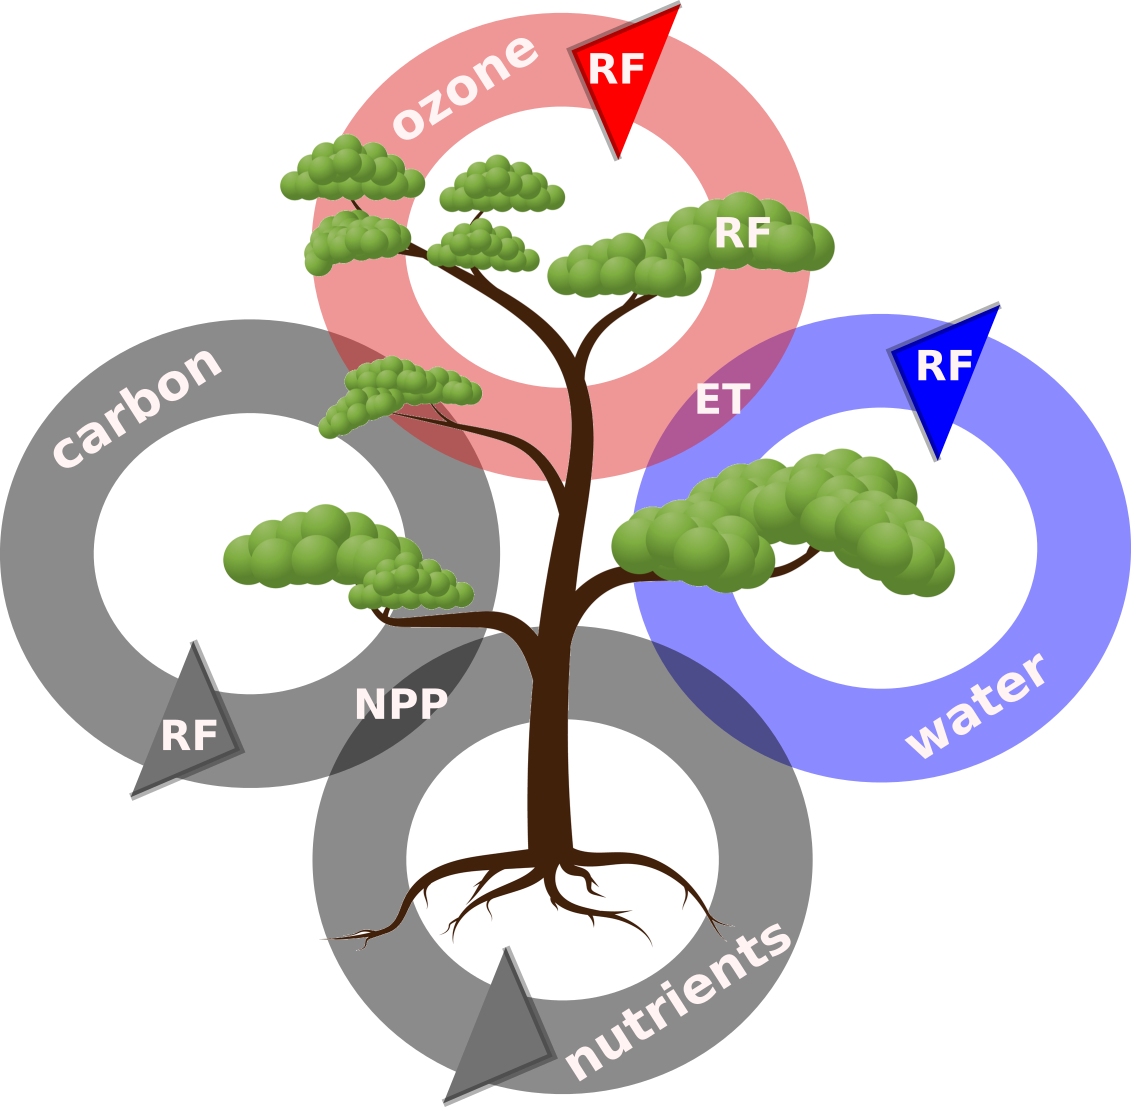
\includegraphics[width=0.48\textwidth]{ozone_es_scheme}
  \caption{Schematic view of the importance of ozone in \glspl{esm}. \textbf{\color{red}Ozone} inflicts damage to vegetation. Ozone affects photosynthesis negatively and hence \gls{npp} (\textbf{\color{darkgray}$\rightarrow$ carbon cycle}). Ozone affects opening and closing of stomata (positively and negatively) and hence \gls{et} of plants (\textbf{\color{blue}$\rightarrow$ water cycle}). Both affect the processing of nutrients (\textbf{\color{darkgray}$\rightarrow$ nutrient cycle}). Ozone damage on vegetation causes positive and negative feedback on tropospheric ozone concentrations and hence on air quality and \gls{rf} \parencite{Nat:Sitch2007}.}
  \label{fig:ozone_esm_scheme}
\end{wrapfigure}

Besides air quality considerations, \textbf{ozone interferes with the climate and Earth system} both directly and indirectly. Directly ozone affects the radiative forcing through its absorbance in both long and short wave bands and hence contributes to climate change. Indirectly ozone affects climate and air quality through ozone impacts on vegetation, which stand at the center of the proposed research. A high \gls{cuo} leads to considerably visible (e.g. necrosis, early senescence) and invisible damage (e.g. reduced photosynthesis, root growth) on vegetation \parencite{GCB:Mills2010}.

\textbf{\color{red}Ozone damage} reduces plant photosynthesis and stomatal conductance. As illustrated in Fig.~\ref{fig:ozone_esm_scheme}, ozone effects on vegetation interfere with several sensitive components of the Earth system. Ozone affects the \textbf{\color{darkgray}carbon cycle} through a reduced photosynthesis capacity and subsequent reduction in \gls{npp} and \gls{gpp}, which has consequences on the \textbf{\color{darkgray}nutrient cycle}. At the same time, physical damage will alter \gls{et} of the plant and hence the \textbf{\color{blue}water cycle}. Depending on the species and severity of damage both a reduction \parencite{Oe:Lombardozzi2012} or an increase (known as stomata sluggishness) have been reported \parencite{SR:Hoshika2015}. Accounting for ozone induced reduction of stomatal conductance and photosynthesis independently, \textcite{BGS:Lombardozzi2012} could improve model projections of changes in \gls{gpp} and transpiration on global scales.

In \textbf{our current understanding of photosynthesis at the plant physiological level}, maximum electron transport rate $\mathrm{J_{max}}$ and maximum carboxylation efficiency $\mathrm{V_{cmax}}$ are key parameters. Empirically it was found that ozone damage leads to a reduction of  $\mathrm{J_{max}}$ and $\mathrm{V_{cmax}}$ \parencite{EJA:Emberson2018}. Because the ratio $\mathrm{J_{max}}$:$\mathrm{V_{cmax}}$ is found to be constant (even under ozone exposure), first order effects of ozone induced damage can be modeled by a relative reduction in $\mathrm{J_{max}}$ or $\mathrm{V_{cmax}}$ alone. A simple linear relationship relates the relative reduction of $\mathrm{J_{max}}$ or $\mathrm{V_{cmax}}$ with the \gls{cuo} \parencites{BGS:Franz2017}{BGS:Franz2018}. \textcite{BGSD:Franz2020} showed that the impact of potential ozone damage on vegetation under climate change scenarios with explicit modeling on the plant physiological level has the potential to suppress projected gains in \gls{gpp} by increased nitrogen fertilization. These results however, have been based on a model without online atmospheric chemistry. \textbf{\color{red}TODO: Ueberleitung zum naechsten Absatz. \color{blue}Vorschlag: Offline coupling of a land model to ozone concentrations provided from another \gls{ccm} as often done lead to inconsistencies due to differing land use and surface roughness and hence dry deposition velocities between the models. Because the provided ozone concentrations from the \gls{ccm} are already in equilibrium with its own dry deposition scheme, a projected reduced uptake due to ozone damage would change the equilibrium concentration if coupled. To study the effects of ozone on vegetation and the feedback on air quality in the most consistent manner, a two-way coupling between land and atmosphere is essential.}\\

\important{Here, we aim to integrate state-of-the-art  process understanding at the vegetation level into a fully coupled \gls{esm} with coupled atmospheric chemistry and state-of-the-art nutrient limited carbon sequestration to study the effects of  ozone damage and thermal stress on vegetation and the resulting feedback on air quality  and climate.}

\section{Own contributions}
\label{sec:contrib}
The importance of ozone in the Earth system extends from large scales (stratospheric chemistry, dynamics, and radiation balance) to the smallest scales (damage on cellular level in plants). Following its trail, the applicant first studied \textbf{ozone depletion and future trends in the stratosphere} using the \gls{ccm} \gls{emac} model. In this respect the research activities primarily focused on future trends of biogenic brominated \gls{vsls} emitted from the ocean and the combined influence of sulfur aerosols \parencite{ACP:Falk2017}. In this study an increase of future ocean-atmosphere flux of brominated \gls{vsls} of $8-10\,\%$ compared to present day was found. A subsequent decrease in the tropospheric mixing ratios of brominated \gls{vsls} and an increase in the lower stratosphere are attributed to changes in atmospheric chemistry and transport and a reduced bromine impact on stratospheric ozone at the end of the 21st century was found  compared to the present day.

The episodic \textbf{\glspl{ode} from the polar spring-time boundary layer} which are associated with suddenly occurring high bromide abundances (bromine explosions) lead the applicants way to model development, precisely the implementation of a bromine release mechanism based on \textcite{ACP:Toyota2011} in the \gls{emac} model. Many aspects of the observed bromine enhancement and associated \glspl{ode} in both polar regions could be reproduced by the model including the applicants extension which paved the way for testing of bromine release mechanisms in a global model \parencite{GMD:Falk2018}.

Subsequently the applicant’s research focused on ozone at lower levels. As a major sink of ozone in the troposphere is dry deposition, the applicant turned her eye towards this problem and integrated the \textbf{variable uptake of ozone by the land biosphere} into the scheme of the Oslo \gls{ctm}~3 \parencite{GMD:Falk2019}. This work has substantially improved ozone dry deposition velocities and abundance to vegetated surfaces in the model, and drew attention to the need for more mechanistic descriptions of dry deposition to non vegetated surfaces.

In the following, the applicants work focused in detail on the representation of \textbf{ozone damage with a special focus on subarctic biomes} \textbf{\color{red}TODO: Add references (IPC Vegetation Taskforce Meeting 2021 and EGU conference contribution 2021)}. The analysis of \gls{do3se} model results revealed that standard parameters optimized for central Europe may lead to significant underestimation of damage inflicted to vegetation acclimated to subarctic climates. \textbf{\color{blue}Added text: The risk posed on subarctic biomes by the progressing climate change and a prolongation of the growing season may therefore be underestimated.}

Last but not least, the applicant studied at the smallest scales the \textbf{process-based impact of ozone on the leaf-level} and implemented the representation of ozone damage on nitrogen utilization in \gls{clm}~5.0 \textbf{\color{red}TODO: Remark first results presented at the \gls{cesm} landmodeling working group meeting 2021)} which is the foundation for the proposed development and analytical work in this project. This work indicated that the impact of ozone damage on \gls{gpp} strongly depends on the occurrence of the damage relative to the seasonal cycle of the vegetation.

\textbf{\color{red}TODO: Add remark that publications of these last two works are in preparation?}


\chapter{Research objective}
\begin{wrapfigure}[17]{R}[0pt]{0.5\textwidth}
  % R - floating; r - h! [narrow lines] <- reduce whitespace below
  \centering
  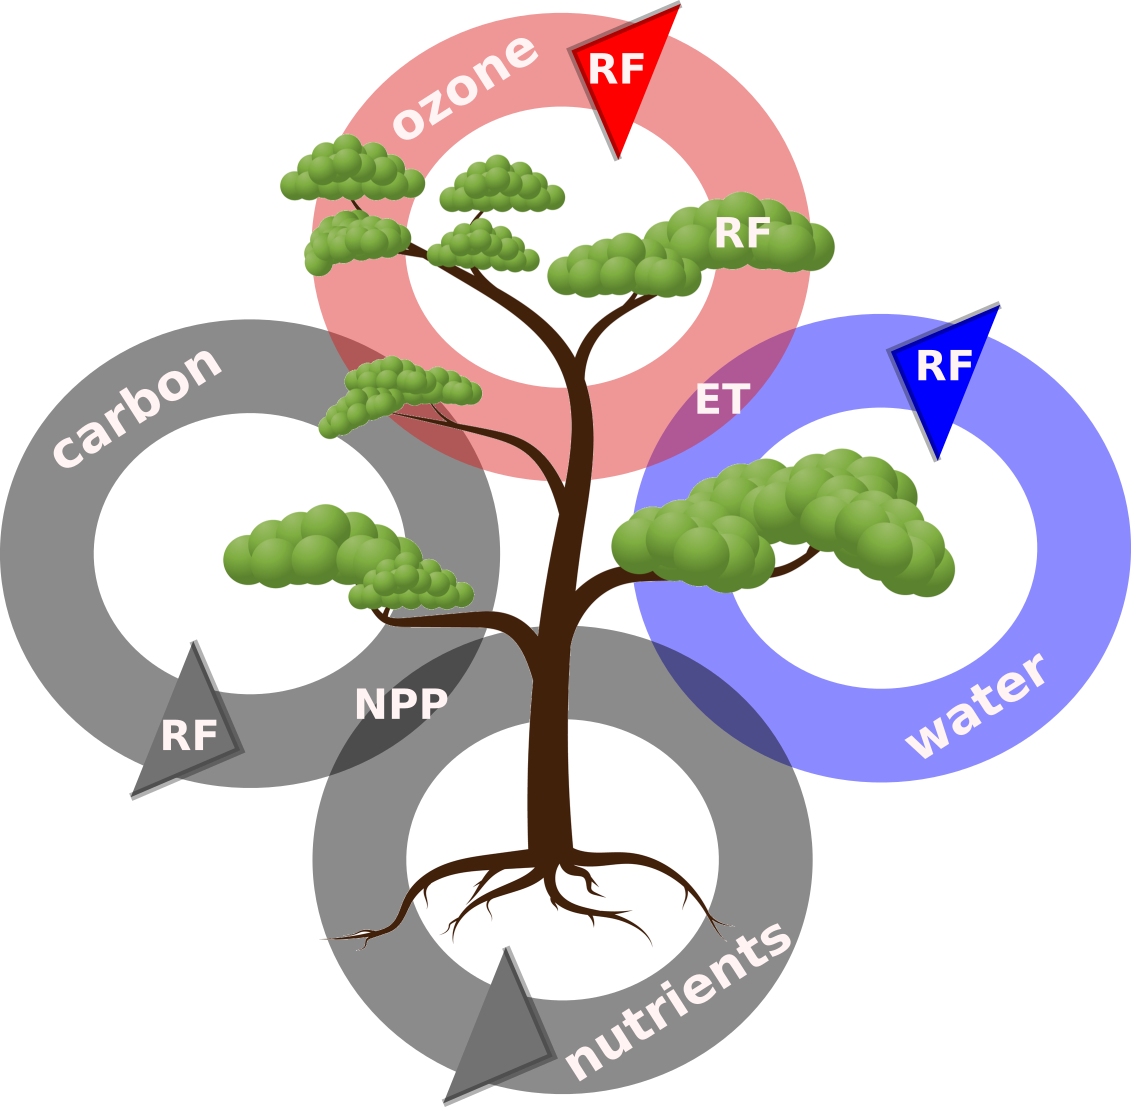
\includegraphics[width=0.48\textwidth]{ozone_es_scheme}
  \caption{Schematic view of the importance of ozone in \glspl{esm}. Ozone inflicts damage to vegetation. Ozone affects photosynthesis negatively and hence \gls{npp} ($\rightarrow$ carbon cycle). Ozone affects opening and closing of stomata (positively and negatively) and hence \gls{et} of plants ($\rightarrow$ water cycle). Both affect the processing of nutrients ($\rightarrow$ nutrient cycle). Ozone damage on vegetation causes positive and negative feedback on tropospheric ozone concentrations and hence on air quality and \gls{rf} \pcite{Nat:Sitch2007}.}
  \label{fig:ozone_es_scheme}
\end{wrapfigure}

Ozone damage reduces plant photosynthesis and stomatal conductance and therefore interferes directly with \gls{npp} and \gls{et} (Fig. 1). Empirically it was found that ozone damage leads to a reduced maximum electron transport rate Jmax and maximum carboxylation efficiency Vcmax (Emberson et al., 2018). Because the ratio Jmax:Vcmax is constant (even under ozone exposure), the main traits of ozone induced damage can be modeled by a relative reduction in Jmax alone (Falk et al., 2021 in preparation, Franz et al., 2018). For this \gls{odina} model, I deduce a linear relationship between an average \gls{cuo} and Jmax relative to a control experiment from a limited number of peer reviewed research articles published in recent years. I take advantage of already existing, scientifically validated modules in \gls{clm}. The integration of \gls{odina} into the existing framework of \gls{clm}~5 is schematically depicted in Fig. 2. \gls{odina} also builds on previous efforts by Lombardozzi et al. (2012, 2013) in collecting a comprehensive database of experimental data for implementation of an ozone damage module. This database is used for model evaluation \gls{odina}. The \gls{odina} model can be used to study ozone effects on the C:N ratio. The purpose of this project is to establish the coupling of \gls{clm}5 to CAM-chem with respect to ozone through dry deposition and evaluate the comprehensive two-way coupling of ozone-vegetation in the light of climate change.


\chapter{Methodes}
\section*{Model description}
The work will be based on the latest release series of the \gls{cesm} and its components, \gls{clm}~5 including \gls{bvoc} emissions (\gls{megan} model \parencite{ACP:Guenther2006}, \gls{cam}~6 with online (super-fast) chemistry (\gls{impact} model, \textcite{JGR:Rotman2004}). 
In the following, I will give a brief account of the most relevant parts of the aforementioned model components of \gls{cesm}, \gls{clm} including \gls{megan}, and \gls{cam}. After that I first present the Lombardozzi model of ozone damage and then elaborate on my more process oriented, new plant physiological model of ozone damage and its integration into \gls{clm}.

In \gls{clm}~5, \textbf{photosynthesis} (and hence the carbon cycle) is tied to \textbf{plant nutrient dynamics} (dark gray cycles depicted in Fig.~\ref{fig:ozone_odina}) which incorporates the \textbf{\gls{fun}} model \parencites{GBC:Fisher2010}{JGR:Brzostek2014}{GCB:Shi2015}. The concept of \gls{fun} is that nitrogen uptake requires an investment of energy (e.g. carbon) and that there is a large number of potential sources of nitrogen available in the environment. The ratio of carbon invested to acquire nitrogen is therefore treated as a cost. \gls{fun} calculates the rate of symbiotic nitrogen fixation for nitrogen passed directly to the plant and passed as inorganic ammonium to the soil \parencite{GBC:Cleveland1999}, separately. Nutrient limitation is represented by a variable plant \ch{C:N} ratio which allows plants to adjust their \ch{C:N} ratio at the leaf level at the cost of nitrogen \parencite{JAMES:Ghimire2016}. The \textbf{\gls{luna}} model \parencites{STE:Xu2019}{GMD:Ali2016} finally links these with photosynthesis. The \gls{luna} model calculates photosynthetic capacity based on optimization of the use of leaf nitrogen under different environmental conditions. \textbf{Stomatal conductance} is based on this \textbf{nitrogen-limited photosynthesis} rather than on potential photosynthesis. The maximum stomatal conductance is obtained from the \textbf{Medlyn stomatal conductance} model \parencite{GCB:Medlyn2011} which is preferred over Ball-Berry-type models \parencite{BallBerry1987} for it’s more realistic behavior at low humidity levels (high vapor pressure deficit) \parencites{PR:Rogers2013}{NP:Rogers2017}.  
As a \textbf{plant hydraulic stress} routine explicitly models water transport through the vegetation according to a simple hydraulic framework \parencite{JAMES:Kennedy2019}, stomatal conductance is also a function of prognostic leaf water potential and hence forced by transpiration. Water stress is calculated as the ratio of attenuated stomatal conductance to maximum stomatal conductance.

\textbf{Biogenic emissions} from vegetation are not integrated into the framework described above but handled by \gls{megan} \textcite{ACP:Guenther2006}. \gls{megan} takes above canopy atmospheric forcing, e.g. solar radiation, temperature, and moisture, and \ch{[CO_2]} as input variables. It only depends on vegetation through \gls{lai} which can be either prescribed (\gls{sp} mode) or dynamic (\gls{bgc} mode) and \gls{pft}. In \gls{clm}~5, \gls{megan} version 2.1 \parencite{GMD:Guenther2012} is implemented. \gls{megan}~2.1 includes 147 chemical compounds which can be subset and grouped together (e.g. \emph{isoprene} = pentane + hexane + heptane + tricyclene). In \gls{clm}, trapping of emissions inside of the canopy is explicitly disabled (escape efficiency set to 1).

In \textbf{\gls{cam}-chem}, \textbf{dry deposition} follows the resistance approach originally described by \textcites{AE:Wesely1989}{AE:Walcek1986} and updated sequentially \parencites{AE:Walmsley1996}{AE:Wesely2000}. All deposited chemical species are mapped to a weighted-combination of ozone and sulfur dioxide depositions to characterize their oxidation potential versus solubility in water. Solubility is dependent on the effective Henry’s law coefficient of the species. All species in the mechanism are per default affected by dry deposition if deposition velocities are defined. 
The computation of \textbf{deposition velocities} (or resistances) ties \gls{cam}-chem to \gls{clm}. Dry deposition velocities vary with \gls{pft}. A grid-averaged velocity is computed as the weighted-mean over all land cover types. The impact from changes in land cover, land use or climate are thus reflected \parencite{GMD:Lamarque2012}. 

\begin{wrapfigure}[]{L}[0pt]{0.5\textwidth}
  % R - floating; r - h! [narrow lines] <- reduce whitespace below [17]
  \centering
  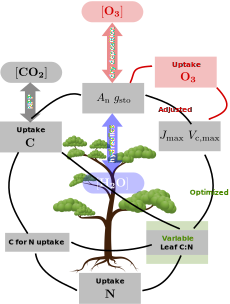
\includegraphics[width=0.48\textwidth]{ozone_luna_scheme}
  \caption{Schematic view of existing process modeling in \gls{clm}~5 and \gls{odina} model in red. Round boxes represent effects on and coupling to atmospheric components of the model (\gls{cam}-chem), e.g. a change in atmospheric concentration of carbon dioxide \ch{[CO_2]}, ozone \ch{[O_3]}, and water vapor \ch{[H_2O]}. Squared boxes represent processes in the land model (\gls{clm}). Plants invest carbon to take up nutrients. A variable carbon to nitrogen ratio (\ch{C:N}) at leaf level determines the optimized electron transport ($\mathrm{J_{max}}$) and carboxylation rate ($\mathrm{V_{cmax}}$). Photosynthesis ($\mathrm{A_n}$) and stomatal conductance ($\mathrm{g_{sto}}$) are dependent on these as well as on plant hydraulics for water transport (blue). Ozone reduces $\mathrm{J_{max}}$ and $\mathrm{V_{cmax}}$ and hence interferes with the whole cycle.
}
  \label{fig:ozone_odina}
\end{wrapfigure}

At present, \textbf{ozone damage} on vegetation is not accounted for by default in \gls{cesm}. There are two reasons for this: 
\begin{enumerate}
  \itemsep0em
\item Ozone fluxes from \gls{cam}-chem are not coupled to \gls{clm} 
\item Running \gls{clm} as stand-alone would necessarily need surface ozone fields which are highly uncertain in available global products (Falk et al. 2021 in preparation).
\end{enumerate}
Ozone damage in \gls{clm}~5 is based on the work of Lombardozzi \parencite{Oe:Lombardozzi2012} which showed an effective decoupling of An and gsto under high \gls{cuo}, with gsto being less sensitive to cumulative uptake of ozone. If taken into consideration this will improve global predictions of GPP and transpiration considerably \parencite{BGS:Lombardozzi2012}, especially in the tropics as also shown by \textcite{ACP:Pacifico2015} and \textcite{ACP:Pacifico2015}. In this implementation, damage coefficients for gsto and An are defined for coniferous, deciduous, and non-woody \glspl{pft}, respectively. \gls{cuo} can be regulated through an uptake threshold $\Phi_\mathrm{th}$. A healing factor is computed based on change in \gls{lai} (growth of new leaves).

The \textbf{\gls{odina}} model, I deduce a linear relationship between an average cumulative uptake of ozone (\gls{cuo}) and $\mathrm{J_{max}}$ relative to a control experiment from a limited number of peer reviewed research articles published in recent years. I take advantage of already existing, scientifically validated modules in \gls{clm} (e.g. \gls{fun}, \gls{luna}). The integration of \gls{odina} into the existing framework of \gls{clm}5 is schematically depicted in Fig. 2. \gls{odina} also builds on previous efforts by \textcites{BGS:Lombardozzi2012}{Oe:Lombardozzi2012}. A comprehensive database of experimental data for implementation of an ozone damage module \parencite{BGS:Lombardozzi2013} will be used for model evaluation of \gls{odina}. The \gls{odina} model can be used to study ozone effects on the \ch{C:N} ratio. The purpose of this project is to establish the coupling of \gls{clm}~5 to \gls{cam}-chem with respect to ozone through dry deposition and evaluate the comprehensive two-way coupling of ozone-vegetation in the light of climate change.


\chapter{Project plan}
\section*{Work packages and tasks}

WP0 - Installation at new workplace\\
T0.1 Getting started and up to speed with institute and settle down in the country\\
T0.2 Setting up \gls{cesm} on institute/national infrastructure\\
WP1 - Model integration\\
T1.1 Finish integration and testing of \gls{odina} in \gls{clm}~5\\
T1.2 Finish and publish development paper on \gls{odina}\\
WP2 - Model coupling (collaboration with \gls{ncar})\\
T2.1 Reverse engineering of dry deposition (understanding model structure and making the right physical choice in which ozone concentration to take)\\
T2.2 Technically coupling \gls{cam}-chem ozone concentrations to \gls{odina}\\
T2.2.a BestCase if ongoing restructuring of couplers in \gls{cesm} is done -> final coupler integration\\
T2.2.b WorstCase: temporary coupling using old infrastructure and come back to 2.2.a at later stage if BestCase is reached within the given time frame\\
WP3 - Model evaluation\\
T3.1 Collection of evaluation data \\
T3.1.1 Site level evaluation (ideally relevant fluxnet sites with observed ozone)\\
T3.1.2 Global scale - surface ozone products (difficult - \gls{ecmwf} \gls{cam} reanalysis sucks) and GPP products (Sentinel satellites? there are issues with \gls{modis} here)\\
T3.2 Write evaluation paper\\
--- BEST CASE SCENARIO----\\
only if WP1 - WP3 are finished within the first 12 months\\
WP4 - Update (tuning) of model parameter\\
T4.1 Implicit ozone effect ought to make it necessary to reevaluate parameters (e.g. $\mathrm{J_{max}}$0 in \gls{luna})\\
T4.2 Implicite “healing” methode\\
WP5 - Production runs and climate projections?\\
T5.1 Run \gls{cesm} coupled of climatological timescales (at least one SSP)\\
T5.2 Study climate impact of ozone damage (gpp, chemistry, air quality...)\\
\\

\begin{wrapfigure}{R}{0.5\textwidth}
  \centering
  \begin{ganttchart}[vgrid, hgrid]{1}{24}
    \gantttitle{ODINA}{24} \\
    \gantttitlelist{1,...,24}{1} \\
    \ganttgroup{WP0}{1}{3} \\
    \ganttbar{T0.1}{1}{3} \\
    \ganttbar{T0.2}{1}{3} \\
    \ganttgroup{WP1}{1}{6} \\
    \ganttbar{T1.1}{1}{3} \\
    \ganttmilestone{Milestone}{3} \ganttnewline
    \ganttbar{T1.2}{2}{6} \\
    \ganttgroup{WP2}{1}{15} \\
    \ganttbar{T2.1}{1}{3} \\
    \ganttbar{T2.2}{1}{3} \\
    \ganttgroup{WP3}{1}{3} \\
    \ganttbar{T3.1}{1}{3} \\
    \ganttbar{T3.2}{1}{3} \\
    \ganttgroup{WP4}{1}{3} \\
    \ganttbar{T4.1}{15}{24} \\
    \ganttbar{T4.2}{15}{24} \\
    %\ganttlinkedbar{Task 2}{3}{7} \ganttnewline
    %\ganttmilestone{Milestone}{7} \ganttnewline
    %\ganttbar{Final Task}{8}{12}
    %\ganttlink{elem2}{elem3}
    %\ganttlink{elem3}{elem4}
  \end{ganttchart}
  \caption{GANTT chart.}
  \label{fig:gantt}
\end{wrapfigure}



%Print the glossary
\printglossaries

\newpage
\printbibliography[env=bibliography]

\end{document}
